\section{Methodology}
\label{sec:methodology}
To establish a distribution on this extremal dependence structure, first we must standardize $\bm{X} \in R^d$
  such that its marginal extreme distributions follow a common form.  Following the work of
  \cite{ferreira2014}, if the marginal distributions $F_{l}$ fall into the domain
  of attraction of some GEV $G_l$, then threshold exceedences for a sufficiently high threshold $b_{l}$
  can be modelled as generalized Pareto $H_l$.  Standardization--transforming threshold exceedences to
  standard Pareto--occurs as
  \begin{equation}
    \label{eqn:standardization}
    Z_l = \left(1 + \xi_l\frac{X_l - b_{t,l}}{a_{t,l}}\right)_{+}^{1/\xi_l}
  \end{equation}
  where $(\cdot)_{+}$ indicates not less than 0. If the quantity inside is less than 0, then the value
  is truncated at 0.  We begin this transformation by establishing the
  marginal thresholds $b_{t,l} := \hat{F}_l^{-1}\left(1 - \frac{1}{t}\right)$, then for those observations
  in excess of the marginal threshold, we fit the scale parameters $a_{t,l}$, and extremal index $\xi_l$
  via maximum likelihood. Note that $z_l > 1$ implies that $x_l > b_{t,l}$, meaning that the observation
  $\bm{x}$ is extreme in the $l$'th dimension.  Note also that $\sup_j Z_j$ follows a simple Pareto
  distribution. Fitting of the marginal extremal index and scale parameters uses only observations in
  excess of the marginal threshold. Following standardization, further analysis is conditional on
  $R \geq 1$.

After standardization and transformation, we have $R\sim\text{Pareto}(1)$, and, independently,
  $\bm{V}\in\mathcal{S}_{\infty}^{d-1}$, the positive orthant of the unit hypersphere under the
  $\mathcal{L}_{\infty}$ norm.  The distribution of $\bm{V}$ effectively describes the dependence
  structure of $\bm{Z}$, so the goal of our analysis subsequently becomes to adequately describe the
  distribution of $\bm{V}$.  We are as yet unaware of any known distributions established with a support
  natively in this space, so we propose projecting a distribution defined on $\mathcal{R}_{+}^{d}$ onto
  $\mathcal{S}_{\infty}^{d-1}$, the unit hypersphere established under the $\mathcal{L}_{\infty}$ norm.

\subsection{Projection onto an arbitrary unit hypersphere}
A hypersphere is a geometric object such that the distance from any point to the center takes a fixed,
  constant value.  The unit hypersphere is a hypersphere where that distance is 1. We can define the
  hypersphere under an arbitrary distance measurement, so let's take the $\mathcal{L}_p$ norm. Let
  the $\mathcal{L}_p$-norm be defined as
  \begin{equation*}
    \lVert {\bf s} \rVert_p = \left(\sum_{l = 1}^d \lvert s_l\rvert^p\right)^{\frac{1}{p}}.
  \end{equation*}
  From this, we establish the $\mathcal{L}_1$ norm as $p = 1$, or the absolute sum, equivalently called
  Manhattan distance; the $\mathcal{L}_2$ norm, as $p = 2$, the Euclidean distance.  From this we
  also establish the $\mathcal{L}_{\infty}$ norm, as
  $\lim\limits_{p\to\infty} \lVert {\bf s} \rVert_p = \max_{l\in\lbrace{1,\ldots,d}}s_l$.

We are interested in the direction, or angular distribution, of vectors described in the positive
  orthant, $\mathcal{R}_{+}^d$.  As we are specifically interested in direction, we can project any
  distribution in $\mathcal{R}_{+}^d$ onto the positive orthant of the unit hypersphere in a
  $\mathcal{L}_p$-norm, denoted as $\mathcal{S}_{p}^{d-1}$.  That is,
  \begin{equation*}
    \mathcal{S}_{p}^{d-1} = \left\lbrace {\bf y} : {\bf y} \in \mathcal{R}_{+}^{d}, \lVert {\bf y}\rVert_{p} = 1\right\rbrace.
  \end{equation*}
  We can project an observation onto this space by dividing said observation by its $p$-norm.  That
  is, let ${\bf x}\in \mathcal{R}_{+}^{d}$, then
  ${\bf y} = {\bf x} / \lVert {\bf x}\rVert_p \in \mathcal{S}_{p}^{d-1}$.  We denote the $d-1$
  to indicate the loss of one degree of freedom relative to the original vector.

So $\mathcal{S}_{1}^{d-1}$ defines the unit simplex, $\mathcal{S}_{2}^{d-1}$ defines the generalization of a
  circle--what we would generally refer to as a hypersphere, and $\mathcal{S}_{\infty}^{d-1}$ the surface of
  the hypercube. The hyperspheres defined by $\mathcal{L}_p$ as $p$ varies have a one to one correspondance
  with eachother, meaning that observations on one can be projected onto another without loss of
  information.

Assuming ${\bf y} \in \mathcal{S}_{p}^{d-1}$, \bruno{sometimes you use bold faces to denote vectors and sometimes you don't. You need to be consistent.}then for finite $p$, $y_d$ can always be represented as a
  function of the other dimensions.  That is,
  \begin{equation*}
    y_d = \left(1 - \sum_{l = 1}^{d-1}y_l^p\right)^{\frac{1}{p}}.
  \end{equation*}
  So the transformation
  \begin{equation*}
    T(x_1,\ldots,x_d) = \left(\pnorm{{\bf x}}{p}, \frac{x_1}{\pnorm{{\bf x}}{p}}, \ldots , \frac{x_{d-1}}{\pnorm{{\bf x}}{p}}\right) = (r,y_1,\ldots,y_{d-1})
  \end{equation*}
  does not lose any information.  The reverse of this transformation,
  \begin{equation*}
    T^{-1}\left(r,y_1,\ldots,y_{d-1}\right) =
      \left(ry_1,\ldots,ry_{d-1},r\left(1 - {\scriptstyle\sum}_{l = 1}^{d-1}y_l^p\right)^{\frac{1}{p}}\right)
  \end{equation*}
  equivalently recovers the original data.  The determinant of the Jacobian of this transformation
  takes the form
  \begin{equation*}
    r^{d-1}\left[\left(1 - \sum_{l = 1}^{d-1}y_l^p\right)^{\frac{1}{p}} +
        \sum_{l = 1}^{d-1}y_l^p\left(1 - \sum_{l=1}^d\right)^{\frac{1}{p} - 1}\right].
  \end{equation*}
  \bruno{There is something missing in this formula}
  Notice a factor of $r^{d-1}$ independent of $p$. We refer to $\bm{y}$ and $r$ as, respectively,
  the angular and radial components of $\bm{x}$.  If we assume a distribution for ${\bf x}$, then
  by transforming to $r, {\bf y}$ and integrating out $r$, we are left with a distribution on solely
  the angular component, or, equivalently, the projection of the vector ${\bf x}$ onto
  $\mathcal{S}_{p}^{d-1}$.

Many of the models we present here follow this form, where we, for reasons to be elaborated, assume
  a $d$-dimensional Gamma distribution on this hypothetical ${\bf x}$. For finite $p$, this has a
  direct benefit in that it is easy to integrate out $r$.  As we saw with the Jacobian computed
  earlier, no matter what $p$, the Jacobian always has a factor of $r^{d-1}$.  With the independent
  Gamma model, $r$ easily integrates out as a gamma distribution.  We can also perform data
  augmentation generating latent $r$'s, and recovering the ability to do independent inference on
  the parameters of those gamma distributions.  We investigated other unidimensional distributions
  with support on $\mathcal{R}_+$ in the hopes we could perform the same dimension reduction with a
  different parameterization, but none offered the flexibility of the Gamma while allowing $r$ to be
  integrated out in closed form.

One might question why we don't use this method to construct a distribution directly on
  $\mathcal{S}_{\infty}^{d-1}$, the unit hypersphere under $\mathcal{L}_{\infty}$.  Put simply, we
  encounter a problem in the transformation.  If we examine the the determinant of the Jacobian
  under the $\mathcal{L}_{p}$ norm, we have a factor along the lines of
  \begin{equation*}
    \left(1 - \sum_{l = 1}^{d-1}y_i^p\right)^{\frac{1}{p} - 1}
  \end{equation*}
  which, if we take the limit as $p$ approaches infinity, if any other $y_l$ than $y_d$ is equal to
  1, then that value approaches $0^{-1}$--an impossibility.  We see a clear breaking point
  between inference conducted on the finite $p$ hypersphere, $\mathcal{S}_{p}^{d-1}$, and the
  $\mathcal{L}_{\infty}$ hypersphere, $\mathcal{S}_{\infty}^{d-1}$. Another way we can recognize
  this issue is from the transformation itself: under $\mathcal{L}_{\infty}$,
  $T^{-1}(r,y_1,\ldots,y_{d-1})$ will not recover $x_1,\ldots,x_d$ if $y_d \neq 1$, or equivalently
  $x_d \neq \max_i x_i$.

With this in mind, the way one might build a distribution on $\mathcal{S}_{\infty}^{d-1}$ that still operates
  in Cartesian coordinates geometry might be to include an equal weighting mixture model, where each
  component of the mixture represents the probability of an observation being on that face, times
  the conditional density of the other dimensions given the face.  That is,
  \begin{equation*}
    f(y) = \sum_{l = 1}^{d}p(y_l = 1)f(y_{-l}\mid y_l = 1)
  \end{equation*}
  Under this interpretation, we can consider $p(y_l = 1) = P(x_l = \max_i x_i)$.  Unfortunately,
  this calculation is not straitforward.

  \makenote{Include arguments from stackexchange thread; cite accordingly}
  \bruno{You need to sharpen the last two paragraphs because I am having a hard time understanding what you are trying to say here.}
  \makenote{I've tried to make it a little more clear.}

Alternatively, one can also map ${\bf y}\in \mathcal{S}_{p}^{d-1}$ into an alternative geometry,
  where we can express those $d-1$ degrees of freedom in a $d-1$ dimensional vector.  On the
  $\mathcal{L}_1$ norm, one might consider isometric or additive logratios\cite{aitchison1982} as
  an appropriate geometry.  On the $\mathcal{L}_2$ norm, we consider spherical coordinates.  This
  directly maps $S_2^{d-1}$ to $[0,\pi/2]^{d-1}$. \cite{nunez2019} follows this course, starting
  with the independent Gamma distribution and still integrating out $r$ to create an angular
  distribution in $[0,\pi/2]^{d-1}$. But we can also construct a distribution directly in this
  space.  Along this idea, via probit transformation we map $[0,\pi/2]^{d-1}$ to
  $(-\infty, \infty)^{d-1}$, and construct a multivariate normal distribution in this geometry.





% EOF


\subsection{Projected Gamma}
\label{method:pg}
The projected gamma distribution, developed in \cite{nunez2019}, is built upon
  the product of $d$ independent gamma distributions.  That is, for
  ${\bf y} = (y_1,\ldots,y_d)^t$, and $y_i\sim\text{Ga}(\alpha_i,\beta_i)$, we
  define our starting point:
\begin{equation}
    f({\bf y}\mid{\bf \alpha},{\bf \beta}) = \prod_{j = 1}^d\text{Ga}(y_j\mid\alpha_j,\beta_j),
\end{equation}
where $\beta$ is specified as a rate parameter.  From that, we transform to
  $d$-dimensional spherical coordinates ${\bf y} \rightarrow (r,{\bf \theta})$
  as
\begin{equation}
  \label{eqn:transform}
  \begin{aligned}
    y_1     &= r\cos\theta_1,\\
    y_2     &= r\sin\theta_1\cos\theta_2\\
            &\vdots\\
    y_{d-1} &= r\sin\theta_1\ldots\sin\theta_{d-2}\\
    y_{d}   &= r\sin\theta_1\ldots\sin\theta_{d-1}
  \end{aligned}
\end{equation}
where $r = \lVert {\bf y}\rVert_{2}$, the euclidean norm of ${\bf y}$.  The
  inverse of this transformation is:
\begin{equation}
  \label{eqn:invtransform}
  \begin{aligned}
    \theta_1     &= \cos^{-1}\left[\frac{y_1}{\lVert y_{1:d}\rVert_2}\right]\\
    \theta_2     &= \cos^{-1}\left[\frac{y_2}{\lVert y_{2:d}\rVert_2}\right]\\
                 &\vdots\\
    \theta_{d-1} &= \cos^{-1}\left[\frac{y_{d-1}}{\lVert y_{(d-1):d}\rVert_2}\right].
  \end{aligned}
\end{equation}
The Jacobian of this transformation is
\begin{equation*}
r^{d-1}\prod_{i = 1}^{d-2}(\sin\theta_i)^{d-1-i}.
\end{equation*}
This creates the distribution over $r,{\bf \theta}$.  The full conditional for
  $r$ takes the form of a Gamma random variable, and we can integrate it out as
  such.  This leaves the \emph{projected gamma distribution},
\begin{equation}
    \text{PG}({\bf \theta}\mid{\bf \alpha},{\bf \beta}) = \frac{\Gamma(A)\beta_d^{\alpha_d}}{B^A\Gamma(a_d}\left(\prod_{j = 1}^{d-1}\frac{\beta_j^{\alpha_j}}{\Gamma(\alpha_j)}(\cos\theta_j)^{\alpha_j - 1}(\sin\theta_j)^{(\sum_{h = j + 1}^d\alpha_h) - 1}\right)\mathcal{I}_{(0,\pi/2)^{d-1}}({\bf \theta})
\end{equation}
where
\begin{equation}
    A = \sum_{j = 1}^d\alpha_j \hspace{1cm}\text{and}\hspace{1cm}B = \beta_1\cos\theta_1 + \sum_{j = 2}^{d-1}\left(\beta_j\cos\theta_j\prod_{i = 1}^{j-1}\sin\theta_i\right) + \beta_d\prod_{j = 1}^d-1\sin\theta_j.
\end{equation}
As is, this model is not identifiable, as taking
  ${\bf \beta}^{(2)} = \alpha {\bf \beta}^{(1)}$ will still yield the same
  distribution of angles. Following \cite{nunez2019}, we have opted to place a
  restriction on $\beta$ such that $\beta_1 := 1$, thus
  ${\bf \beta} = (1, \beta_2, \ldots, \beta_d)^t$.

Inference on this model can take two forms: ${\bf \alpha}$ and ${\bf \beta}$ in
  this form can not be broken down into known-form full conditionals, so we can
  conduct a Metropolis Hastings step for every component, or do a joint proposal
  Metropolis Hastings step for all components at once.  Alternatively, using
  $f(r,{\bf \theta})$, we recognize that $\alpha_i\mid r$ is independent of
  $\alpha_j\mid r$, so we can sample the latent $r$ and conduct independent
  Gibbs steps for each component.  Further, in sampling the $\alpha_j$'s, we can
  integrate out $\beta_j$. Within the Gibbs sampler, we sample $r$, then each
  $\alpha_j\mid r$, then each $\beta_j\mid r, \alpha_j$.  This leads to fast
  convergence, with the only Metropolis Hastings step being for the
  $\alpha_j$'s.  Both $r$ and the $\beta_j$'s are Gamma distributed.

For simplicity, let ${\bf y^{\prime}} = r^{-1}{\bf y}$.  That is,
  ${\bf y^{\prime}}$ is a function of the angular data--from~\eqref{eqn:transform},
  ${\bf y^{\prime}} = {\bf y}/r$, the projection of the ${\bf y}$ vector onto
  the unit hypersphere. We generate a latent $r$, and their product is the
  latent ${\bf y}$.  Given ${\bf y}$, the posterior distributions for
  $(\alpha_i, \beta_i)$, $(\alpha_j,\beta_j)$, $i\neq j$ are independent.

As~\cite{nunez2019} shows, the projected gamma distribution is a flexible model
  for representing data on the positive orthant of the unit hypersphere.  As such,
  given our application restricts us to this domain, one can see that this might be a
  natural choice of distribution for our purpose.

\begin{figure}[h!]
  \centering
  \label{fig:vanillamix}
  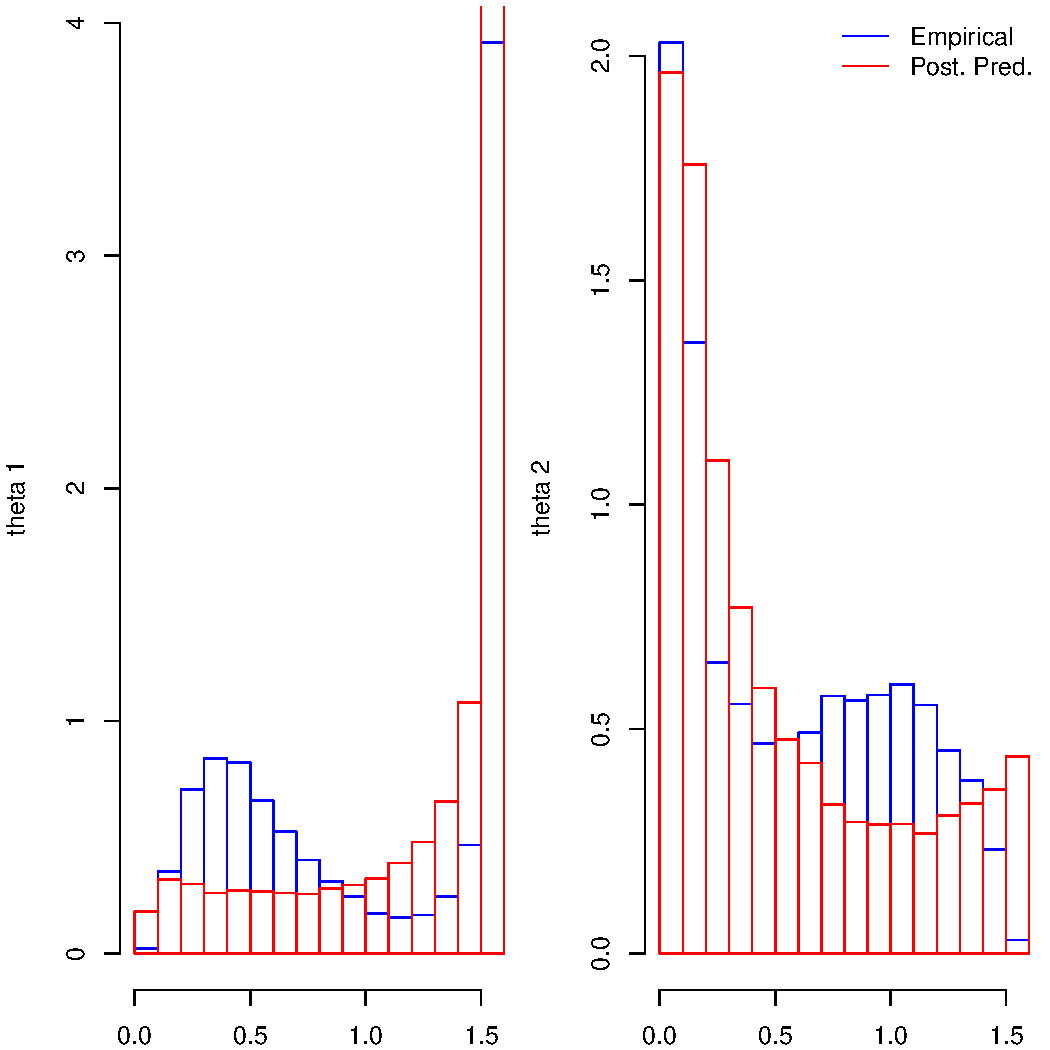
\includegraphics[width=5in]{./images/justification_for_more_complex_models}
  \caption{Histograms of Empirical vs Posterior-predictive angular data originating
            from a simulated 3-dimensional gamma dataset.}
\end{figure}

However, as flexible as it is, it alone is not sufficient for our purpose.  Supposing
  a given dataset is the result of two or more generating distributions, then using a
  a single distribution to represent this dataset becomes untenable.  In Figure~\ref{fig:vanillamix}
  we see the empirical distribution a 2-component mixture of projected gammas, plotted
  against the posterior predictive distribution of a projected gamma model fitted to
  that dataset.  As we can see, it has trouble representing the nuances of the two
  component mixture.


% EOF


\subsection{Alternative Geometries}
An alternative to this projected distribution model, one method we might consider would be to map
  to an alternative geometry, where we can express those $d-1$ degrees of freedom in a $d-1$
  dimensional vector.  In such a space, we can assign whatever model seems appropriate without the
  degrees of freedom restriction necessary in the projected gamma model.  Choosing what $\mathcal{L}_p$
  norm hypersphere we start mapping from identifies what possible geometries we might use.  For instance,
  on the $\mathcal{L}_1$ norm, a possible geometry might be isometric or additive
  logratios~\citep{aitchison1982}.  On the $\mathcal{L}_2$ hypersphere, we consider spherical
  coordinate transformation. Let $\bm{y} \in \mathcal{S}_{2}^{d-1}$. Then, we transform $\bm{y}$
  to spherical coordinates as
  \begin{equation*}
    \theta_l = \arccos\frac{y_l}{\pnorm{\bm{y}_{l:d}}{2}},
  \end{equation*}
  for $l = 1,\ldots, d-1$. That is, the arccosine of the ratio of the mass of a given element,
  versus the \emph{combined} mass of that and subsequent elements.  If $x_l = 0$, and
  $\pnorm{\bm{x}_{l:d}}{2} > 0$, then $\theta_l = \frac{\pi}{2}$, indicating that all the mass was
  in later dimensions.  Alternatively, if $\theta_l = 0$, then that indicates all the mass was in
  the current element.  One can see here that ordering of the axes has a great effect on the
  resulting coordinates.  The inverse of this transformation takes the form:
  \begin{equation}
    \label{eqn:spherical}
    \begin{aligned}
      y_1 &= \cos\theta_1\\
      y_l &= \left[\prod_{k = 1}^{l-1}\sin\theta_k\right]\cos\theta_l \hspace{1cm}\text{for } l = 2,\ldots,d-1\\
      y_d &= \prod_{k = 1}^{d-1}\sin\theta_k
    \end{aligned}
  \end{equation}
  \cite{nunez2019} use this transformation to project a product of Gammas distribution in
  $\mathcal{R}^d$ onto $[0,2\pi]^{d-1}$ Alternatively, we then map these spherical coordiates via
  probit transformation to $(-\infty,\infty)$ to consider a multivariate normal distribution.
  \makenote{Rewrite Paragraph}

% EOF



\subsection{Normal model built on Probit representation of Spherical Coordinate Space}
\label{method:npprobitnorm}
The transformation in Equation~\ref{eqn:transform} provides us a mapping from $S_{2}^{d-1}$ to a
  $d-1$ dimensional cube, $[0, \pi/2]$.  Building on this transformation allows us to represent
  the data using a true $d-1$ dimensional distribution, rather than generating a latent parameter
  to induce a $d$ dimensional distribution, as we do with all the gamma based models.

A canonical choice of distribution in this space might be to further transform to $(-\infty, \infty)$
  via marginal probit or logit transformation, and represent the data as multivariate normal.  We try
  that here.   Let $W_i = \text{Probit}(2\theta_i /\pi)$--that is, scale $\theta_i$ to the unit
  interval, then conduct a probit transformation on it to result in $W_i \in (-\infty, \infty)$.
  Then we establish a multivariate normal distribution on $W$. As we are expecting data to descend
  from a mixture of distributions, we place a DP prior on the multivariate normal kernel
  distribution.  The centering distribution of the DP prior is the product of a multivariate normal
  and inverse Wishart distribution; and we place multivarite normal and inverse Wishart priors on
  these parameters.  As before, we place a gamma prior on the DP concentration parameter $\eta$.
  \begin{equation}
    \begin{aligned}
                W_i &\sim \mathcal{N}_{d-1}\left(\mu_i, \Sigma_i\right)\\
    \mu_i, \sigma_i &\sim G_i\\
                G_i &\sim \text{DP}(\eta, G_0(\mu_i,\Sigma_i\mid\mu_0,\Sigma_0))\\
                    &\hspace{1cm}G_0(\mu_i,\Sigma_i\mid\mu_0,\Sigma_0) &=
                      \mathcal{N}_{d-1}(\mu_i\mid\mu_0,\Sigma_0)\text{IW}(\Sigma\mid\nu,\psi)\\
              \mu_0 &\sim \mathcal{N}_{d-1}\left({\bf u},{\bf S}\right)\\
           \Sigma_0 &\sim \text{IW}(\nu_0,\psi_0)\\
               \eta &\sim \text{Ga}(\alpha, \beta)
    \end{aligned}
  \end{equation}
There is an advantage in that for inference on $\mu_i, \mu_0, \Sigma_i$, and $\Sigma_0$ this model
  is completely conjugate.  However, while the transformation employed in Equation~\ref{eqn:transform}
  is one to one, small deviations in different dimensions on $S_{\infty}^{d-1}$ have vastly different
  effects on the resulting transformed variables.  This induced distortion may result in an inferior
  model, when evaluating on $S_{\infty}^{d-1}$.  We will be evaluating this model as representative
  of models on the $d-1$ dimensional coordinate space, and comparing it against other models, after
  projecting back onto $S_{\infty}^{d-1}$.

Another disadvantage of this model is the need to compute $d-1$-dimensional matrix determinants
  and inversions.  If we consider that inversion is a $\mathcal{O}(n^3)$ operation, we face the real
  problem of computation time climbing astronomically as the number of dimensions grows.  We are
  currently evaluating this model on 8 and 46 dimensions, we can see that those operations on 46
  dimensions will take around 190 times longer than on 8 dimensions.  This presents a problem if we
  want to run this model in any reasonable time scale.

% EOF


% EOF
